% Options for packages loaded elsewhere
\PassOptionsToPackage{unicode}{hyperref}
\PassOptionsToPackage{hyphens}{url}
%
\documentclass[
  man,floatsintext]{apa6}
\usepackage{amsmath,amssymb}
\usepackage{iftex}
\ifPDFTeX
  \usepackage[T1]{fontenc}
  \usepackage[utf8]{inputenc}
  \usepackage{textcomp} % provide euro and other symbols
\else % if luatex or xetex
  \usepackage{unicode-math} % this also loads fontspec
  \defaultfontfeatures{Scale=MatchLowercase}
  \defaultfontfeatures[\rmfamily]{Ligatures=TeX,Scale=1}
\fi
\usepackage{lmodern}
\ifPDFTeX\else
  % xetex/luatex font selection
\fi
% Use upquote if available, for straight quotes in verbatim environments
\IfFileExists{upquote.sty}{\usepackage{upquote}}{}
\IfFileExists{microtype.sty}{% use microtype if available
  \usepackage[]{microtype}
  \UseMicrotypeSet[protrusion]{basicmath} % disable protrusion for tt fonts
}{}
\makeatletter
\@ifundefined{KOMAClassName}{% if non-KOMA class
  \IfFileExists{parskip.sty}{%
    \usepackage{parskip}
  }{% else
    \setlength{\parindent}{0pt}
    \setlength{\parskip}{6pt plus 2pt minus 1pt}}
}{% if KOMA class
  \KOMAoptions{parskip=half}}
\makeatother
\usepackage{xcolor}
\usepackage{graphicx}
\makeatletter
\def\maxwidth{\ifdim\Gin@nat@width>\linewidth\linewidth\else\Gin@nat@width\fi}
\def\maxheight{\ifdim\Gin@nat@height>\textheight\textheight\else\Gin@nat@height\fi}
\makeatother
% Scale images if necessary, so that they will not overflow the page
% margins by default, and it is still possible to overwrite the defaults
% using explicit options in \includegraphics[width, height, ...]{}
\setkeys{Gin}{width=\maxwidth,height=\maxheight,keepaspectratio}
% Set default figure placement to htbp
\makeatletter
\def\fps@figure{htbp}
\makeatother
\setlength{\emergencystretch}{3em} % prevent overfull lines
\providecommand{\tightlist}{%
  \setlength{\itemsep}{0pt}\setlength{\parskip}{0pt}}
\setcounter{secnumdepth}{-\maxdimen} % remove section numbering
% Make \paragraph and \subparagraph free-standing
\makeatletter
\ifx\paragraph\undefined\else
  \let\oldparagraph\paragraph
  \renewcommand{\paragraph}{
    \@ifstar
      \xxxParagraphStar
      \xxxParagraphNoStar
  }
  \newcommand{\xxxParagraphStar}[1]{\oldparagraph*{#1}\mbox{}}
  \newcommand{\xxxParagraphNoStar}[1]{\oldparagraph{#1}\mbox{}}
\fi
\ifx\subparagraph\undefined\else
  \let\oldsubparagraph\subparagraph
  \renewcommand{\subparagraph}{
    \@ifstar
      \xxxSubParagraphStar
      \xxxSubParagraphNoStar
  }
  \newcommand{\xxxSubParagraphStar}[1]{\oldsubparagraph*{#1}\mbox{}}
  \newcommand{\xxxSubParagraphNoStar}[1]{\oldsubparagraph{#1}\mbox{}}
\fi
\makeatother
% definitions for citeproc citations
\NewDocumentCommand\citeproctext{}{}
\NewDocumentCommand\citeproc{mm}{%
  \begingroup\def\citeproctext{#2}\cite{#1}\endgroup}
\makeatletter
 % allow citations to break across lines
 \let\@cite@ofmt\@firstofone
 % avoid brackets around text for \cite:
 \def\@biblabel#1{}
 \def\@cite#1#2{{#1\if@tempswa , #2\fi}}
\makeatother
\newlength{\cslhangindent}
\setlength{\cslhangindent}{1.5em}
\newlength{\csllabelwidth}
\setlength{\csllabelwidth}{3em}
\newenvironment{CSLReferences}[2] % #1 hanging-indent, #2 entry-spacing
 {\begin{list}{}{%
  \setlength{\itemindent}{0pt}
  \setlength{\leftmargin}{0pt}
  \setlength{\parsep}{0pt}
  % turn on hanging indent if param 1 is 1
  \ifodd #1
   \setlength{\leftmargin}{\cslhangindent}
   \setlength{\itemindent}{-1\cslhangindent}
  \fi
  % set entry spacing
  \setlength{\itemsep}{#2\baselineskip}}}
 {\end{list}}
\usepackage{calc}
\newcommand{\CSLBlock}[1]{\hfill\break\parbox[t]{\linewidth}{\strut\ignorespaces#1\strut}}
\newcommand{\CSLLeftMargin}[1]{\parbox[t]{\csllabelwidth}{\strut#1\strut}}
\newcommand{\CSLRightInline}[1]{\parbox[t]{\linewidth - \csllabelwidth}{\strut#1\strut}}
\newcommand{\CSLIndent}[1]{\hspace{\cslhangindent}#1}
\ifLuaTeX
\usepackage[bidi=basic]{babel}
\else
\usepackage[bidi=default]{babel}
\fi
\babelprovide[main,import]{english}
% get rid of language-specific shorthands (see #6817):
\let\LanguageShortHands\languageshorthands
\def\languageshorthands#1{}
% Manuscript styling
\usepackage{upgreek}
\captionsetup{font=singlespacing,justification=justified}

% Table formatting
\usepackage{longtable}
\usepackage{lscape}
% \usepackage[counterclockwise]{rotating}   % Landscape page setup for large tables
\usepackage{multirow}		% Table styling
\usepackage{tabularx}		% Control Column width
\usepackage[flushleft]{threeparttable}	% Allows for three part tables with a specified notes section
\usepackage{threeparttablex}            % Lets threeparttable work with longtable

% Create new environments so endfloat can handle them
% \newenvironment{ltable}
%   {\begin{landscape}\centering\begin{threeparttable}}
%   {\end{threeparttable}\end{landscape}}
\newenvironment{lltable}{\begin{landscape}\centering\begin{ThreePartTable}}{\end{ThreePartTable}\end{landscape}}

% Enables adjusting longtable caption width to table width
% Solution found at http://golatex.de/longtable-mit-caption-so-breit-wie-die-tabelle-t15767.html
\makeatletter
\newcommand\LastLTentrywidth{1em}
\newlength\longtablewidth
\setlength{\longtablewidth}{1in}
\newcommand{\getlongtablewidth}{\begingroup \ifcsname LT@\roman{LT@tables}\endcsname \global\longtablewidth=0pt \renewcommand{\LT@entry}[2]{\global\advance\longtablewidth by ##2\relax\gdef\LastLTentrywidth{##2}}\@nameuse{LT@\roman{LT@tables}} \fi \endgroup}

% \setlength{\parindent}{0.5in}
% \setlength{\parskip}{0pt plus 0pt minus 0pt}

% Overwrite redefinition of paragraph and subparagraph by the default LaTeX template
% See https://github.com/crsh/papaja/issues/292
\makeatletter
\renewcommand{\paragraph}{\@startsection{paragraph}{4}{\parindent}%
  {0\baselineskip \@plus 0.2ex \@minus 0.2ex}%
  {-1em}%
  {\normalfont\normalsize\bfseries\itshape\typesectitle}}

\renewcommand{\subparagraph}[1]{\@startsection{subparagraph}{5}{1em}%
  {0\baselineskip \@plus 0.2ex \@minus 0.2ex}%
  {-\z@\relax}%
  {\normalfont\normalsize\itshape\hspace{\parindent}{#1}\textit{\addperi}}{\relax}}
\makeatother

\makeatletter
\usepackage{etoolbox}
\patchcmd{\maketitle}
  {\section{\normalfont\normalsize\abstractname}}
  {\section*{\normalfont\normalsize\abstractname}}
  {}{\typeout{Failed to patch abstract.}}
\patchcmd{\maketitle}
  {\section{\protect\normalfont{\@title}}}
  {\section*{\protect\normalfont{\@title}}}
  {}{\typeout{Failed to patch title.}}
\makeatother

\usepackage{xpatch}
\makeatletter
\xapptocmd\appendix
  {\xapptocmd\section
    {\addcontentsline{toc}{section}{\appendixname\ifoneappendix\else~\theappendix\fi: #1}}
    {}{\InnerPatchFailed}%
  }
{}{\PatchFailed}
\makeatother
\usepackage{csquotes}
\ifLuaTeX
  \usepackage{selnolig}  % disable illegal ligatures
\fi
\usepackage{bookmark}
\IfFileExists{xurl.sty}{\usepackage{xurl}}{} % add URL line breaks if available
\urlstyle{same}
\hypersetup{
  pdftitle={Exploring Aspects of Social Interaction using Machine Learning},
  pdfauthor={Nele-Pauline Suffo1, Pierre-Etienne Martin2, Daniel Haun2, \& Manuel Bohn1, 2},
  pdflang={en-EN},
  hidelinks,
  pdfcreator={LaTeX via pandoc}}

\title{Exploring Aspects of Social Interaction using Machine Learning}
\author{Nele-Pauline Suffo\textsuperscript{1}, Pierre-Etienne Martin\textsuperscript{2}, Daniel Haun\textsuperscript{2}, \& Manuel Bohn\textsuperscript{1, 2}}
\date{}


\shorttitle{Exploring Aspects of Social Interaction using Machine Learning}

\authornote{

The authors made the following contributions. Nele-Pauline Suffo: Conceptualization, Writing - Original Draft Preparation, Writing - Review \& Editing; Manuel Bohn: Writing - Review \& Editing, Supervision.

Correspondence concerning this article should be addressed to Nele-Pauline Suffo, Universitätsallee 1, 21335 Lüneburg. E-mail: \href{mailto:nele.suffo@leuphana.de}{\nolinkurl{nele.suffo@leuphana.de}}

}

\affiliation{\vspace{0.5cm}\textsuperscript{1} Institute of Psychology in Education, Leuphana University Lüneburg\\\textsuperscript{2} Max Planck Institute for Evolutionary Anthropology}

\abstract{%
tbd
}



\begin{document}
\maketitle

\section{Introduction}\label{introduction}

\section{Methodology}\label{methodology}

The Quantex dataset includes

\subsection{Dataset Description}\label{dataset-description}

\subsubsection{Statistics}\label{statistics}

The Quantex dataset contains a total of 197.20 hours of video footage from 503 video recordings, collected by 76 children aged 3 to 5 years (M=4.53, SD=0.81). The children were grouped into three age categories, with 167 videos being recorded of children age 3, 180 videos for children age 4, and 156 videos at age 5. Individual recording durations vary widely, ranging from 10.43 to 391.18 minutes per child (M=155.68, SD=82.62). Figure \ref{fig:quantex-minutes-per-child} illustrates the detailed distribution of recording lengths, reflecting the diversity in individual contributions to the dataset.

\begin{figure}

{\centering 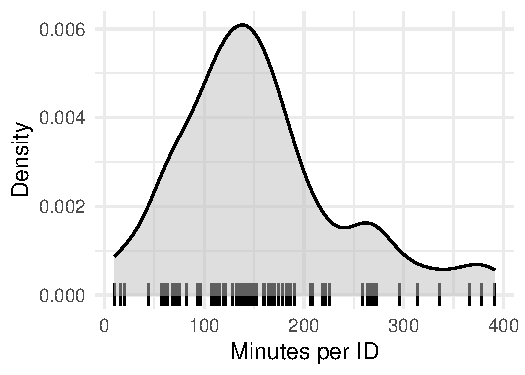
\includegraphics{Quantex_interaction_paper_files/figure-latex/quantex-minutes-per-child-1} 

}

\caption{Video recording duration (in minutes) per Child in the Quantex Dataset.}\label{fig:quantex-minutes-per-child}
\end{figure}

\subsubsection{Annotation Strategy}\label{annotation-strategy}

The dataset annotations cover four key elements: persons, faces, objects the child interacts with, and gaze direction. Gaze information identifies whether a detected person's gaze is directed toward the child or not. For every detected person (or reflection of a person, such as in a mirror) and face, additional attributes like age and gender are collected. Objects are categorized into six distinct groups: book, screen, animal, food, toy, and kitchenware, with an additional category for other objects. The dataset focus is on detecting and labeling instances of (social) interaction and engagement through these key categories. The annotation strategy is displayed in Figure \ref{fig:camera-cvat-activity-classes}.

\begin{figure}

{\centering 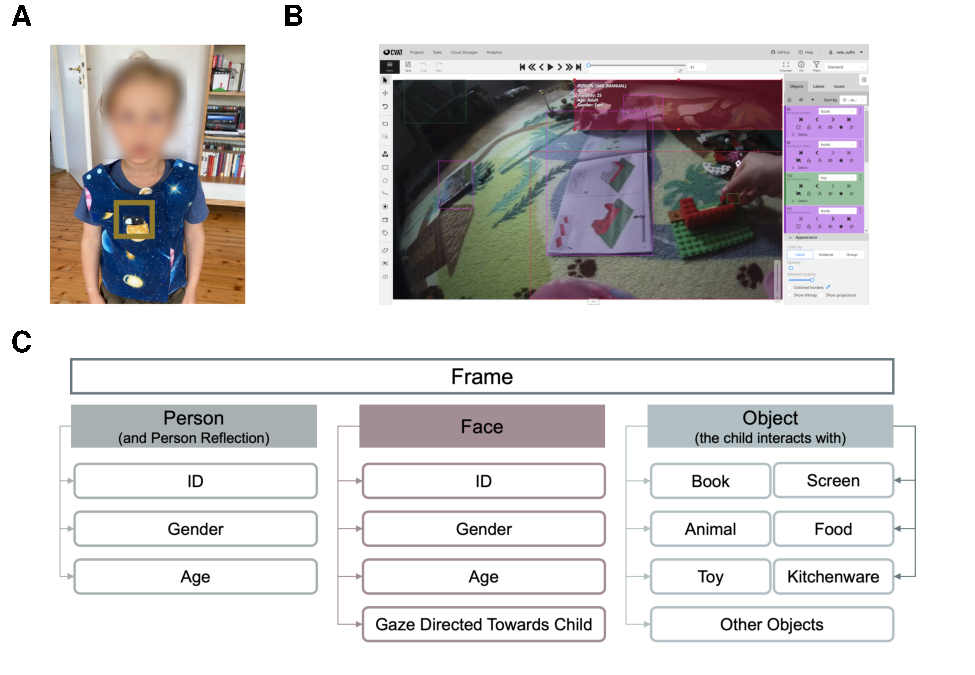
\includegraphics{Quantex_interaction_paper_files/figure-latex/camera-cvat-activity-classes-1} 

}

\caption{\textbf{A} – Vest with the embedded camera worn by the children, \textbf{B} – CVAT platform utilized for video annotation, \textbf{C} – Annotation strategy in the Quantex dataset.}\label{fig:camera-cvat-activity-classes}
\end{figure}

\subsection{Data Collection}\label{data-collection}

This study collected egocentric video recordings from 76 children, aged 3 to 5 years, over a span of 73 months. Participating families lived in a mid-sized city in Germany. To capture the children's everyday experiences, a wearable vest equipped with a camera was used, as shown in figure \ref{fig:camera-cvat-activity-classes}. The camera, a \emph{PatrolEyes WiFi HD Infrared Police Body Camera}, provided high-definition video (1920x1080p at 30 fps) with a 140-degree wide-angle lens and also recorded audio. Children were free to move around and engage in their usual activities at home without any interference or instructions given to their parents.

\subsection{Data Preprocessing}\label{data-preprocessing}

For the video data, the annotation strategy required persons, faces, and objects to be labeled even when only partially visible, as long as key features such as facial landmarks (e.g., nose, eye, or mouth) or parts of a person or object were clearly visible. Frames that were too blurry due to movement were marked as ``noise'' and excluded from further analysis. Additionally, frames where the child was not wearing the camera, as well as any scenes containing nudity, were also labeled as noise and removed from the dataset. To prepare the video data for analysis, one frame per second was annotated, corresponding to every 30th frame in the video. Similarly, every 30th raw frame was extracted from the annotated video files. No preprocessing was applied to the audio data, which was used in its raw form for analysis.

\subsection{Automated Analysis Pipeline}\label{automated-analysis-pipeline}

\subsubsection{Person Detection}\label{person-detection}

\subsubsection{Face Detection}\label{face-detection}

\subsubsection{Gaze Classification}\label{gaze-classification}

\subsubsection{Voice Detection and Classification}\label{voice-detection-and-classification}

\subsection{Feature Extraction}\label{feature-extraction}

\section{Results}\label{results}

\subsection{Presence of Aspects of Social Interaction}\label{presence-of-aspects-of-social-interaction}

\subsubsection{Presence of a Person}\label{presence-of-a-person}

\subsubsection{Presence of a Face}\label{presence-of-a-face}

\subsubsection{Presence of Gaze Directed at the Child}\label{presence-of-gaze-directed-at-the-child}

\subsubsection{Presence of Language}\label{presence-of-language}

\subsection{Co-occurrence of Aspects of Social Interaction}\label{co-occurrence-of-aspects-of-social-interaction}

\section{General Discussion}\label{general-discussion}

We present the ChildLens dataset, a unique egocentric video-audio dataset that documents children's everyday experiences, spanning a wide age range of 3 to 5 years. This dataset is particularly distinctive due to its diversity in terms of the number of children it includes and the variety of activity labels it covers. By focusing on both visual and auditory data, the ChildLens dataset provides comprehensive annotations for a broad spectrum of key activities, offering rich insights into children's social and behavioral interactions in naturalistic settings. This makes it a valuable resource for studying developmental processes in children, with a focus on their cognitive, emotional, and social growth.

In comparison to other freely available datasets, the ChildLens dataset stands out due to its broad age span and diverse set of activity labels. Most other datasets focus either on toddlers, are limited to dyadic interactions or were recorded in lab settings, with all of them lacking a comprehensive range of activity labels. Furthermore, most of these datasets either capture only audio or video, missing the multimodal aspect crucial for understanding children's everyday experiences. In contrast, ChildLens includes naturalistic recordings from children's home environments, over an extended period, and features a variety of activity types. The dataset also captures whether children are engaged in activities alone or with others and provides detailed demographic information about all individuals involved. This comprehensive approach enables a deeper and more holistic understanding of children's interactions and developmental trajectories.

The usefulness of the ChildLens dataset is demonstrated by its successful application to well-established models. For example, the pretrained Voice-Type Classifier for audio transcription achieves performance comparable to previous datasets, while the Boundary-Matching Network (BMN) produces robust results for activity localization, consistent with its performance on other datasets. These results indicate that the ChildLens dataset's annotations align well with model predictions, highlighting its quality and potential for multimodal research. Moreover, the successful application of these models demonstrates how the dataset can support and automate the analysis of children's everyday activities.

Expanding the potential for multi-method approaches, activity localization could be further enhanced by incorporating object identification, allowing for better tracking of the objects children interact with during daily routines, as demonstrated in adult-focused studies (Kazakos, Huh, Nagrani, Zisserman, \& Damen, 2021). Research by Bambach et al. (Bambach, Lee, Crandall, \& Yu, 2015) also emphasizes the importance of hand detection in egocentric video for activity recognition. Their work on using Convolutional Neural Networks for hand segmentation highlights how such techniques can differentiate activities, offering a deeper understanding of children's interactions and behaviors.

The integration of visual and auditory data in the ChildLens dataset enables a more detailed and comprehensive understanding of children's daily experiences. Complex activities such as pretend play and reading a book, which require both audio and video for accurate detection, exemplify the strength of this multimodal approach. While previous studies, such as those analyzing disfluencies in children's speech during computer game play (Yildirim \& Narayanan, 2009), have demonstrated that combining visual and auditory information can improve performance, few studies have explored this in the context of children's naturalistic activities. With ChildLens, the combination of naturalistic data and multimodal analysis creates new opportunities for in-depth insights into children's cognitive, emotional, and social development, particularly for activities best captured through both modalities.

Despite its strengths, one limitation of the ChildLens dataset is the class imbalance, especially in underrepresented activity classes, which could affect model training and evaluation. More frequent activities, such as ``child talking'' (7447 instances, 649 minutes) and ``playing with object'' (317 instances, 1371 minutes), dominate the dataset, while less common activities like ``dancing'' (2 instances, 0.57 minutes) and ``making music'' (2 instances, 2.13 minutes) are scarcely represented. Similarly, activities like ``pretend play'' (59 instances, 158.84 minutes) and ``reading a book'' (81 instances, 328.70 minutes) appear less frequently. This imbalance may lead to skewed model performance, making it harder to accurately classify rare activities. Possible solutions to this challenge could involve merging rare activity classes into broader categories or excluding them from model training, though these approaches may reduce the dataset's diversity. Other methods, such as resampling or augmentation, could help balance the dataset and improve model performance (Alani, Cosma, \& Taherkhani, 2020; Spelmen \& Porkodi, 2018).

In addition to class imbalance, another potential limitation is the sampling bias. Since the recordings are largely influenced by parental decisions about when and how often activities are captured, certain activities or settings may be overrepresented or underrepresented based on these preferences. Furthermore, the dataset primarily focuses on families from a mid-sized German city, limiting its geographic and cultural diversity. Expanding the dataset to include a broader range of families from different regions and cultures would enhance its generalizability and applicability to various research contexts.

The study of children's everyday experiences is crucial for understanding their cognitive, emotional, and social development. These daily interactions provide important insights into how children learn, grow, and engage with their environment. The ChildLens dataset makes a valuable contribution to this field by offering a rich multimodal resource that captures the complexities of children's lives in naturalistic settings. With its comprehensive annotations and potential to automate the analysis of children's activities, the dataset enables researchers to gain deeper and more detailed insights into children's development. By making such analyses more efficient and accessible, the ChildLens dataset creates new opportunities for understanding the complexities of early childhood development and provides a foundation for future research in this area.

\newpage

\section{References}\label{references}

\begingroup
\setlength{\parindent}{-0.5in}
\setlength{\leftskip}{0.5in}

\phantomsection\label{refs}
\begin{CSLReferences}{1}{0}
\bibitem[\citeproctext]{ref-alaniClassifyingImbalancedMultimodal2020}
Alani, A. A., Cosma, G., \& Taherkhani, A. (2020). Classifying {Imbalanced Multi-modal Sensor Data} for {Human Activity Recognition} in a {Smart Home} using {Deep Learning}. \emph{2020 {International Joint Conference} on {Neural Networks} ({IJCNN})}, 1--8. Glasgow, United Kingdom: IEEE. \url{https://doi.org/10.1109/IJCNN48605.2020.9207697}

\bibitem[\citeproctext]{ref-bambachLendingHandDetecting2015}
Bambach, S., Lee, S., Crandall, D. J., \& Yu, C. (2015). Lending {A Hand}: {Detecting Hands} and {Recognizing Activities} in {Complex Egocentric Interactions}. \emph{2015 {IEEE International Conference} on {Computer Vision} ({ICCV})}, 1949--1957. Santiago, Chile: IEEE. \url{https://doi.org/10.1109/ICCV.2015.226}

\bibitem[\citeproctext]{ref-kazakosLittleHelpMy2021}
Kazakos, E., Huh, J., Nagrani, A., Zisserman, A., \& Damen, D. (2021). With a {Little Help} from my {Temporal Context}: {Multimodal Egocentric Action Recognition}. \url{https://doi.org/10.48550/ARXIV.2111.01024}

\bibitem[\citeproctext]{ref-spelmenReviewHandlingImbalanced2018}
Spelmen, V. S., \& Porkodi, R. (2018). A {Review} on {Handling Imbalanced Data}. \emph{2018 {International Conference} on {Current Trends} Towards {Converging Technologies} ({ICCTCT})}, 1--11. Coimbatore: IEEE. \url{https://doi.org/10.1109/ICCTCT.2018.8551020}

\bibitem[\citeproctext]{ref-yildirimAutomaticDetectionDisfluency2009}
Yildirim, S., \& Narayanan, S. (2009). Automatic {Detection} of {Disfluency Boundaries} in {Spontaneous Speech} of {Children Using Audio}\&\#x2013;{Visual Information}. \emph{IEEE Transactions on Audio, Speech, and Language Processing}, \emph{17}(1), 2--12. \url{https://doi.org/10.1109/TASL.2008.2006728}

\end{CSLReferences}

\endgroup

\newpage

\section{Appendix}\label{appendix}

\subsection{List of ChildLens Activity Classes}\label{list-of-childlens-activity-classes}

The dataset contains the following list of activities.

\begin{enumerate}
\def\labelenumi{\arabic{enumi}.}
\tightlist
\item
  \textbf{playing with object}: The child is playing with an object, such as a toy or a ball.
\item
  \textbf{playing without object}: The child is playing without an object, such as playing hide and seek or catch.
\item
  \textbf{pretend play}: The child is engaged in imaginative play, such as pretending to be a doctor or a firefighter.
\item
  \textbf{watching something}: The child is watching a movie, TV show, or video on either a screen or a device.
\item
  \textbf{reading book}: The child is reading a book or looking at pictures in a book.
\item
  \textbf{child talking}: The child is talking to themselves or to someone else.
\item
  \textbf{other person talking}: Another person is talking to the child.
\item
  \textbf{overheard speech}: Conversations that the child can hear but is not directly involved in.
\item
  \textbf{drawing}: The child is drawing or coloring a picture.
\item
  \textbf{crafting things}: The child is engaged in a craft activity, such as making a bracelet or decoration.
\item
  \textbf{singing / humming}: The child is singing or humming a song or a melody.
\item
  \textbf{making music}: The child is playing a musical instrument or making music in another way.
\item
  \textbf{dancing}: The child is dancing to music or moving to a rhythm.
\item
  \textbf{listening to music / audiobook}: The child is listening to music or an audiobook.
\end{enumerate}

\subsection{List of ChildLens Location Classes}\label{list-of-childlens-location-classes}

\begin{enumerate}
\def\labelenumi{\arabic{enumi}.}
\tightlist
\item
  livingroom
\item
  playroom
\item
  bathroom
\item
  hallawy
\item
  other
\end{enumerate}

\subsection{Activity Class Statistics}\label{activity-class-statistics}

\begin{table}[tbp]

\begin{center}
\begin{threeparttable}

\caption{\label{tab:activity-classes-statistics}Number of video instances and the total duration (in minutes).}

\begin{tabular}{llll}
\toprule
Category & \multicolumn{1}{c}{Activity Class} & \multicolumn{1}{c}{Instance Count} & \multicolumn{1}{c}{Total Duration (min)}\\
\midrule
Audio & Child talking & 7447 & 649.10\\
 & Other person talking & 6113 & 455.29\\
 & Overheard Speech & 1898 & 299.44\\
 & Singing/Humming & 277 & 82.00\\
 & Listening to music/audiobook & 68 & 222.14\\
Video & Watching something & 2 & 5.09\\
 & Drawing & 62 & 374.91\\
 & Crafting things & 26 & 109.14\\
 & Dancing & 2 & 0.57\\
Multimodal & Playing with object & 317 & 1371.06\\
 & Playing without object & 25 & 28.87\\
 & Pretend play & 59 & 158.84\\
 & Reading a book & 81 & 328.70\\
 & Making music & 3 & 2.13\\
\bottomrule
\end{tabular}

\end{threeparttable}
\end{center}

\end{table}


\end{document}
